\chapter{Introduction}\label{ch:Introduction}



%\section{Motivation}
%Why is the topic of interest? 
%New technology
%    IoT development
%    Massive number of devices
%    5G

The market of cellular technologies is changing and the need for a new type of technology has arisen. This is the need for \gls{LPWA} networks. \gls{LPWA} networks are classified by long battery lifetime, low-cost units and a large number of devices.  With the development of \gls{LPWA} networks,  an increased focus has come to the massive part of communication. This is especially true for the development of 5G and other \gls{IoT} technologies. The massive aspect relates to the number of devices trying to connect to the network in a given area.  In \gls{LPWA} networks the density of devices is several folds larger compared to normal cellular networks. In 2016 a report estimated that 0.4 billion devices were of the \gls{LPWA} type. It went on and predicted an increase to 1.5 billion by 2021, equivalent to a yearly growth rate of 27 \% \citep{mobi-report}. This change sets some requirements that are not achievable with existing systems. Several technologies exist to accommodate this.


Generally, the new technologies are classified as cellular network based solution and proprietary solutions. The most renowned solutions is seen on \autoref{fig:IoT_protocol_overview}. All these technologies are competing to be the main standard of LPWA systems. 
%\textbf{Objective}

\tikzsetnextfilename{IoT_fig}
\begin{figure}[H]
\centering
%\resizebox{\textwidth}{!}{
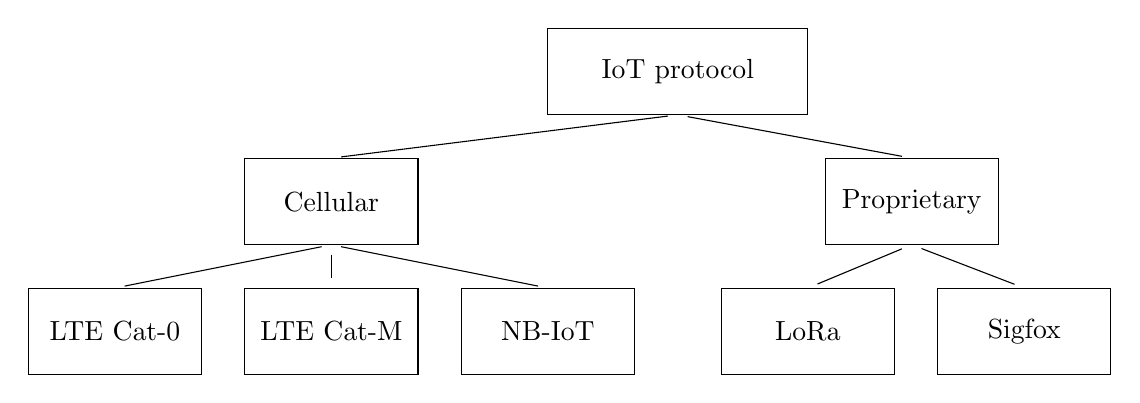
\begin{tikzpicture}[scale=0.11]
\draw  (10,100) rectangle (40,90);
\node at (25,95) {IoT protocol};
\draw  (-25,85) rectangle (-5,75);
\node at (-15,80) {Cellular};
\draw  (42,85) rectangle (62,75);
\node at (52,80) {Proprietary};

\draw  (-50,70) rectangle (-30,60);
\node at (-40,65) {LTE Cat-0};
\draw  (-25,70) rectangle (-5,60);
\node at (-15,65) {LTE Cat-M};
\draw  (0,70) rectangle (20,60);
\node at (10,65) {NB-IoT};
\draw  (30,70) rectangle (50,60);
\node at (40,65) {LoRa};
\draw  (55,70) rectangle (75,60);
\node at (65,65) {Sigfox};


%\draw  (-2,47) ellipse (4 and 4);
%\draw (-2,51) -- (48,51) -- (48,43) -- (-2,43);
%\node at (-2,47) {A};
%\node [anchor=west] at (8,47) {Reliability};
%
%\draw  (-2,35) ellipse (4 and 4);
%\draw (-2,39) -- (48,39) -- (48,31) -- (-2,31);
%\node at (-2,35) {B};
%\node [anchor=west] at (8,35) {Energy consumption};
%
%\draw  (-2,23) ellipse (4 and 4);
%\draw (-2,27) -- (48,27) -- (48,19) -- (-2,19);
%\node at (-2,23) {C};
%\node [anchor=west] at (8,23) {Massiveness};

\node (v1) at (25,90) {};
\node (v2) at (-15,85) {};
\node (v3) at (52,85) {};
\node (v4) at (-15,75) {};
\node (v5) at (-40,70) {};
\node (v6) at (-15,70) {};
\node (v7) at (10,70) {};
\node (v8) at (52,75) {};
\node (v9) at (40,70) {};
\node (v10) at (65,70) {};
\draw  (v1) edge (v2);
\draw  (v1) edge (v3);
\draw  (v4) edge (v5);
\draw  (v4) edge (v6);
\draw  (v4) edge (v7);
\draw  (v8) edge (v9);
\draw  (v8) edge (v10);
\end{tikzpicture}%}
\caption{LPWA protocol overview.}
\label{fig:IoT_protocol_overview}
\end{figure}



\section{Problem Analysis}
%What is the problem?
%    Many standards 
%    Not really tested
%    Nothing really deployed
%    Unity
%Why do we have the problem?
%    New technology
%    Money
%    Competitiveness
%Problem statement!

The technologies in question are still in development. As an effect of this, the metrics found for the different protocols, are to the authors' knowledge based on a theoretic approach and not on actual measurements. 

\begin{table}[H]
\centering
\resizebox{\textwidth}{!}{%
\begin{tabular}{|l|l|l|l|l|l|}
\hline
\textbf{Feature}            & \textbf{LoRa}           & \textbf{Sigfox}               & \textbf{LTE Cat-1} & \textbf{LTE-M}    & \textbf{NB-IoT} \\ \hline
Modulation                  & SS Chirp                   & UNB/GSK/BPSK                & OFDMA              & OFDMA                 & OFDMA           \\ \hline
Rx bandwidth                & 500-125 kHz                & 100 Hz                      & 20 MHz             & 20-1.4 MHz            & 200 KHz         \\ \hline
Data Rate                   & 290 bps – 50 Kbps          & 100 bps / 8 bytes max        & 10 Mbps               & 200 kbps – 1 Mbps     & 20 Kbps         \\ \hline
Max output power            & 20 dBm                     & 20 dBm                      & 23 – 46 dBm        & 23/30 dBm             & 20 dBm          \\ \hline
\begin{tabular}[c]{@{}l@{}}Battery lifetime \\ (2000 mAh)\end{tabular}& 105 months ($\sim$9 years) & 90 months (7.5 years)  &   & 18 months (1.5 years) &   \\ \hline
Link budget                 & 154 dB                     & 151 dB                      & 130 dB+            & 146 dB                & 150 dB          \\ \hline
Security                    & Yes                        & No                          & Yes                & Yes                   &                 \\ \hline
\end{tabular}%
}
\caption{Comparison of performance metrics between cellular solutions and proprietary solutions \citep{NB_comp}}%http://www.3glteinfo.com/lora/lora-advantages/}
\label{tab:tech_comparison1}
\end{table}



% Please add the following required packages to your document preamble:
% \usepackage{graphicx}
%\begin{table}[H]
%\centering
%%\resizebox{\textwidth}{!}{%
%\begin{tabular}{|l|l|l|l|l|}
%\hline
%\textbf{Feature}   & \textbf{\begin{tabular}[c]{@{}l@{}}Release 8\\ Cat 4\end{tabular}} & \textbf{\begin{tabular}[c]{@{}l@{}}Release 8\\ Cat 1\end{tabular}} & \textbf{\begin{tabular}[c]{@{}l@{}}Release 13\\ LTE-M\end{tabular}} & \textbf{\begin{tabular}[c]{@{}l@{}}Release 13\\ NB-IoT\end{tabular}} \\ \hline
%Downlink speed     & 150 Mbps                                                           & 10 Mbps                                                            & 384 kbps - 1Mbps                                                    & 170-250 kbps                                                         \\ \hline
%Uplink speed       & 50 Mbps                                                            & 5 Mbps                                                             & 384 kbps - 1Mbps                                                    & 50-144 kbps                                                          \\ \hline
%Number of antennas & 2                                                                  & 2                                                                  & 1                                                                   & 1                                                                    \\ \hline
%Duplex mode        & Full duplex                                                        & Full duplex                                                        & Full or Half duplex                                                 & Half duplex                                                          \\ \hline
%Receive bandwidth  & 20 MHz                                                             & 20 MHz                                                             & 1.4 MHz                                                             & 200 kHz                                                              \\ \hline
%Transmit power     & 23 dBm                                                             & 23 dBm                                                             & 20 dBm                                                              & 23 dBm                                                               \\ \hline
%Modem complexity   & 100 \%                                                             & 80 \%                                                              & 20 \%                                                               & \textless15 \%                                                       \\ \hline
%Voice              & Yes                                                                & Yes*                                                               & Yes                                                                 & No                                                                   \\ \hline
%Mobility           & Full                                                               & Full                                                               & Limited                                                             & \begin{tabular}[c]{@{}l@{}}Fixed-Idle\\ Mode Only\end{tabular}       \\ \hline
%\end{tabular}%
%%}
%\caption{Comparison of cellular solutions \citep{CAT_comp}} %https://www.digi.com/blog/cellular/introduction-to-lte-m-cellular-technology/
%\label{tab:tech_comparison2}
%\end{table}

It can be seen from \autoref{tab:tech_comparison1}, that the different technologies have different properties. The main differences are the bandwidth of the receiver as well as the battery lifetime. 

As none of the protocols have been deployed at a large scale, it brings up different concerns. This is because the massiveness in question is several times larger than anything seen before.  An IoT developer chooses an LPWA protocol based on performance metrics. These metrics relate to three domains: reliability, energy consumption, and massiveness. 

The reliability refers to the error rate of the system. This is important, as the devices might be placed e.g. in a sewer. If this is the case the \gls{MCL} could be very high, which is very influential for the error rate. Another factor to consider here is the latency of the system.\\
The energy consumption is important as the main power grid might not be available for the device. It would then have to run on an internal power source. The reason for this again has to do with the placement of the device. A concern is that the device is placed in a hard to get to location and the number of replacements of the battery and device should be small.\\
The massiveness is important as the density of devices is increased several folds. Each device might not take up a lot of bandwidth, but share number of devices, means for use cases, that is new and untested so far.

The general scenario of an LPWA system is a large number of devices. Each transmitting a small, not latency critical, payload at regular intervals e.g. smart meters, household equipment, and surveillance. %The aim is to have long battery lifetime,  The reliability is in most cases not critical, but depending on the re-transmission scheme chosen a low reliability might result in unnecessary stress on the network. This might decrease performance for both massiveness and energy consumption of the devices. 


%One of the aims of \gls{IoT} devices is a battery lifetime of around 10 years, to achieve this requirement for the energy consumption is, of course, a key metric. With the scope of billions of devices, several metrics in regards to the massiveness will also be extremely important. Because of the long lifetime coupled with the extreme number of devices the reliability also needs to be very high as it is not feasible to replace devices quickly. 
%\todo{Either add payload as an extra domain or rewrite the part about reliability}

This leads to the problem statement:
\begin{center}
\textbf{As the IoT market is still under development, the proposed protocols need to be evaluated based on several metrics for the reliability, energy consumption and massiveness. This evaluation will allow IoT developers to determine which IoT protocol is best suited for their target application.}
\end{center}

%Several different metrics can be tested for each of the domains some are protocol specific others while others are more general. Examples of performance metrics are:
%
%\begin{itemize}
%    \item[\textbf{A}] \textbf{Massiveness}
%    \begin{itemize}
%        \item Time to connect vs. connection request per second 
%        \item Data rate vs. number of users
%        \item Spectrum use vs. number of users
%        \item Interference level vs. number of users
%    \end{itemize}        
%    \item[\textbf{B}] \textbf{Energy consumption}
%    \begin{itemize}
%        \item Energy consumption vs. data rate
%        \item Energy consumption vs. coverage level
%        \item Energy consumption vs. operation mode
%        \item Energy consumption vs. number of UEs
%        \item Energy consumption vs. cellular protocol
%        \item Energy consumption cellular vs. proprietary
%    \end{itemize}
%    \item[\textbf{C}] \textbf{Reliability}
%    \begin{itemize}
%        \item Delay
%        \item \gls{BER} vs. \gls{SINR}/\gls{MCL} vs. protocol
%    \end{itemize}
%\end{itemize}


\section{Solution Analysis}
%What has been done before?
%    Last thesis
%    Some test into battery lifetime
%    Theoretic calculations
%What could be a solution for the problem?
%    An IoT emulator
%    Comparison of theoretic metrics
%    Choose blindly
%    Deploy a test case
%What are we working with and why?
%    An IoT emulator
%    Massiveness
%    Power
%Why not reliability



The idea for this project is to design an emulator combining both software and hardware. The emulator should test how the protocols perform in the different domains. For this purpose, emulation of a massive number of low-performance \gls{IoT} devices is needed. This idea is illustrated on \autoref{fig:intro_fig}. Implementation of a signal processing method, that allows changing to different channel models, would be optimal. The aim is to provide a customizable emulator, that evaluates performance metrics for the different \gls{IoT} protocols. 

\tikzsetnextfilename{intro_fig}
\begin{figure}[H]
\centering
\resizebox{0.5\textwidth}{!}{
\begin{tikzpicture}

\draw  (-3,3.5) rectangle (-0.5,0.5);
\draw (-1,3.5) -- (-1,4) -- (-3.5,4) -- (-3.5,1) -- (-3,1);
\draw (-1.5,4) -- (-1.5,4.5) -- (-4,4.5) -- (-4,1.5) -- (-3.5,1.5);
\node at (-1.75,2) {Device};
\draw  (1.5,3) rectangle (4.5,1);
\node at (3,2) {Channel};

\draw (7.5,1)  -- (7,0) -- (8,0) -- (7.5,1) -- (7.5,1.5);
\draw  (7.5,2) ellipse (0.5 and 0.5);
\draw  plot[smooth, tension=1] coordinates {(7.1,2.75) (6.75,2) (7.1,1.25)};
\draw  plot[smooth, tension=1] coordinates {(6.8,2.75) (6.45,2) (6.8,1.25)};
\node at (7.5,-0.5) {BSE};

\draw (7.5,-3.5)  -- (7,-4.5) -- (8,-4.5) -- (7.5,-3.5) -- (7.5,-3);
\draw  (7.5,-2.5) ellipse (0.5 and 0.5);
\draw  plot[smooth, tension=1] coordinates {(7.1,-1.75) (6.75,-2.5) (7.1,-3.25)};
\draw  plot[smooth, tension=1] coordinates {(6.8,-1.75) (6.45,-2.5) (6.8,-3.25)};
\node at (7.5,-5) {BSE};

\draw (7.5,5.5)  -- (7,4.5) -- (8,4.5) -- (7.5,5.5) -- (7.5,6);
\draw  (7.5,6.5) ellipse (0.5 and 0.5);
\draw  plot[smooth, tension=1] coordinates {(7.1,7.25) (6.75,6.5) (7.1,5.75)};
\draw  plot[smooth, tension=1] coordinates {(6.8,7.25) (6.45,6.5) (6.8,5.75)};
\node at (7.5,4) {BSE};
\draw (-0.5,2) -- (1.5,2);
\draw (4.5,2) node (v1) {} -- (6.4,2);

\draw (v1) -- (6.5,-2) -- (v1) -- (6.5,6) ;
\end{tikzpicture}}
\caption{Conceptual visualisation of the emulator.}
\label{fig:intro_fig}
\end{figure}

An earlier project has focused on building a software emulator for the LTE protocol \citep{thesis_report}. The idea there was to use a single radio and then emulate multiple devices in software. They used SRS LTE UE as a baseline and added multiple functionalities on top \citep{thesis_report}. This project will leverage on this work to build a \gls{MDE}.

%\textbf{Limits of project} \todo{check this when it is decided to to do track 1 or 2}\\
As it is a huge endeavor to build an emulator fulfilling the desired concepts, the focus will be only on the core principles. When making an emulator, it generally only works for a single protocol, as designing it for several protocols would be very time-consuming. Thus the focus is on developing functionalities for a single protocol instead. Another factor is the project will build upon existing software. Because designing either of the \gls{BSE} or \gls{IoT} device emulators could easily be its own project. The choice of protocol for the project is based on different factors seen in \autoref{tab:protocol_decision}.

\begin{table}[H]
\centering
\resizebox{\textwidth}{!}{
\begin{tabular}{|c|c|c|c|c|c|} \hline
                    & \textbf{LTE Cat-0}& \textbf{LTE Cat-M}    & \textbf{NB-IoT}    & \textbf{LoRa}    & \textbf{Sigfox}    \\ \hline
Licensed spectrum    & Yes                & Yes                    & Yes                & No            & No                \\ \hline
\gls{BS} emulator    &  Amarisoft &  Amarisoft & {\begin{tabular}{c}  Amarisoft \\ SRS \end{tabular}} & \begin{tabular}{c}  The Things Industries \\ * LoRa Server \end{tabular} &   \\ \hline

Device emulator    &  & {\begin{tabular}{c}  Amarisoft \\ Asiatelco \\ AT\&T \\ Digi \\ Fibocom \\ Gemalto \\ H3C \\ Huawei \\ LinkLabs \\ Longsung \\ Meig \\ Mobiletek \\ Multitech \\ Neoway \\ NimbeLink \\ pycom \\ Quectel \\ Sierra Wireless \\ SimCom \\ Skyworks \\ Telit \\ u-blox \\ ZTEWelink  \end{tabular}} & {\begin{tabular}{c}  Amarisoft \\ Cheerzing \\ CMCC \\ Digi \\ H3C \\ Lierda \\ Longsung \\ Meig \\ Mobiletek \\ Mokuai \\ Neoway \\ pycom \\ Quectel \\ Sierra Wireless \\ SimCom \\ Skyworks \\ Telit \\ u-blox \\ ZTEWelink \\ SRS \end{tabular}} & {\begin{tabular}{c}  The Things Industries \\  Miromico \\  Telit \end{tabular}} &    {\begin{tabular}{c}   Murata \\  Telit \\ * Telefonicaid \end{tabular}} \\ \hline
Modem complexity    & High                 & Middle                 & Middle             & Middle         & Low                \\ \hline
\end{tabular}}
\raggedright \scriptsize{ * Open source solutions} 
\caption{Commercial solutions available for the different protocols \citep{UE_list, Amarisoft_solutions, SRS_solutions, LORA_solutions, Things_solutions, Mira_solutions, Telit_solutions, telefonicaid_solutions, murata_solutions}.}%The solutions presented is found from google searches and might not show a complete image of available solutions.}
\label{tab:protocol_decision}
\end{table}

%Based on \autoref{tab:protocol_decision} the \gls{NB-IoT} protocol is chosen. This is based on the fact it uses the licensed spectrum as well as the solutions available. Also, it is chosen to primarily look at the massiveness aspect of the protocol. \todo{check with germans comments}%check this again before hand-in}

When looking at \autoref{tab:protocol_decision} it can be seen that for \gls{LTE} Cat-0 no device emulator was found. This has to do with the development of \gls{LTE} Cat-M and \gls{NB-IoT}, which shares most of the same properties but are more specialized to the \gls{IoT} market. It can also be seen that for both \gls{LTE} Cat-M and \gls{NB-IoT} multiple device emulators exist. The reason for this is that both protocols are cellular protocols developed by \gls{3GPP}. This is very desired by the industry for various reasons. For \gls{LoRa} there exists both \gls{BS} and device emulators, as it is also one of the most used proprietary protocols on the market. For the Sigfox protocol, no \gls{BS} emulators have been found. 

Based on these investigations it is chosen to use the \gls{NB-IoT}. There are two reasons for this, it has a lot of emulators already developed and the bandwidth is less than LTE CAT-M. The desire for a small bandwidth is based on the before mentioned project. The project found that decreasing the bandwidth increased the number of devices the system could support \citep{thesis_report}. 


To make the most realistic emulation, the final solution needs to work in real time, which sets some limitations performance wise. One of the problems associated with real-time computation is the computational capacity. This implies that the emulator might not be able to handle several thousand devices simultaneously, as the deployed system is required to. This is further explored in \autoref{ch:mass_test}.

Another limit that has been set for the project, is to not focus on the reliability domain. This is done partly because it is believed to be the domain with the least concern of the three domains for NB-IoT and partly because any one of the domains, are large enough to fill out the scope of a single project. The focus in the project is split between the energy consumption and massiveness domains and in both cases, further limits still need to be set. For the massiveness domain, the channel will only consist of a path loss component. As this is all that is needed to validate a proof of concept emulator. The primary concern here is also the key functionalities and an API is not prioritized. For the energy consumption, an existing emulator will be used for the BSE and an engineering device is used as a test device. The focus further limited to only show the influence of a few key parameters for the battery lifetime. %The emulator is designed in modules, which in the future could be put together to one complete system.  

This outline the scope of the project. To achieve this an overview of the \gls{NB-IoT} protocol is given in \autoref{ch:NB-IoT}. Here the network structure, protocol layers, and network access are explained. The rest of the report is divided between the two domains. \autoref{ch:MassOver} and \autoref{ch:mass_test} focus on the massive domain. Here the work done to build a \gls{MDE} as well as show the capabilities of the \gls{MDE} is explained. The goal for the MDE is to make a proof of concept emulator, emulating more than 15 devices as this was the limit in the previous project. \autoref{ch:BatTest} focus on the energy consumption domain. The idea here is to use a simple model to estimate the battery lifetime of an NB-IoT device and show the influence of selected parameters. The results found from each of these domains, along with the problems encountered are discussed in \autoref{ch:dics}. The final evaluation is described in \autoref{ch:con}, together with a proposed future direction for the work done in this project. 